\documentclass[handout, 10pt]{beamer}

%\usepackage[backend=bibtex,firstinits=true,style=verbose-inote,citestyle=authortitle]{biblatex}
\usepackage{bm}
\usepackage{graphicx}
\usepackage{subcaption}
\usepackage{amsmath}
\usepackage{amsfonts}
\usepackage{makecell}
\usepackage{filecontents}
\usepackage{biblatex}
% \newcommand{\expect}[2][]{
\ifthenelse{\equal{#1}{}}{
\mathbb{E}\left[#2\right]
}{
\underset{#1}{\mathbb{E}}\left[#2\right]
}}

\newcommand{\cov}[2][]{
\ifthenelse{\equal{#1}{}}{
\text{Cov}\left[#2\right]
}{
\underset{#1}{\text{Cov}}\left[#2\right]
}}


\newcommand{\var}[2][]{
\ifthenelse{\equal{#1}{}}{
\text{Var}[#2]
}{
\underset{#1}{\text{Var}}[#2]
}}

\newcommand{\loss}[2][]{
\ifthenelse{\equal{#1}{}}{
\mathcal{L}(#2)
}{
\mathcal{L}_{#1}(#2)
}}

\newcommand{\kl}[2]{
\text{D}_\text{KL}[#1 \parallel #2]
}

\newcommand{\R}{\mathbb{R}}
%\newcommand{\Prob}{\mathbb{P}}

\newcommand{\1}[1]{\mathds{1}\{#1\}}


%\usecolortheme{dolphin}
\setbeamertemplate{navigation symbols}{}
\setbeamertemplate{section in toc}{\inserttocsectionnumber.~\inserttocsection}

\begin{filecontents*}{references.bib}
@article{StateOfSparsity,
  author    = {Trevor Gale and
               Erich Elsen and
               Sara Hooker},
  title     = {The State of Sparsity in Deep Neural Networks},
  journal   = {CoRR},
  volume    = {abs/1902.09574},
  year      = {2019},
  url       = {http://arxiv.org/abs/1902.09574},
  archivePrefix = {arXiv},
  eprint    = {1902.09574},
  timestamp = {Tue, 21 May 2019 18:03:40 +0200},
  biburl    = {https://dblp.org/rec/journals/corr/abs-1902-09574.bib},
  bibsource = {dblp computer science bibliography, https://dblp.org}
}
\end{filecontents*}

\addbibresource{references.bib}


\title{The State of Sparsity in Deep Neural Networks\footnote{\citepaper{StateOfSparsity}}}
%\subtitle{}
%\author{Ivan Skorokhodov}
%\date{}
%\logo{
\includegraphics[height=1cm]{images/ipavlov-logo.png}}

\newcommand{\citepaper}[1]{\citetitle{#1} by \citeauthor{#1}}

%\graphicspath{{./images}}

%\usetheme{lucid}
\begin{document}

\begin{frame}
    \titlepage
\end{frame}

\begin{frame}{Overview}
    \begin{itemize}
        \item\pause Authors benchmark different pruning techniques on different large-scale tasks
        \item\pause Their benchmarks demonstrate that ``state-of-the-art'' techniques often lose to simple baselines
        \item\pause They failed to reproduce lottery ticket hypothesis in a large-scale scenario
    \end{itemize}
\end{frame}

\begin{frame}{Sparsity techniques}
    \begin{itemize}
        \item\pause \textit{Magnitude pruning}: gradually mask out more and more weights during training based on their magnitudes.
        \item\pause \textit{Variational dropout}: train a bayesian model with gaussian posterior and remove weights with large variance.
        \item\pause \textit{$l_0$ regularization}: train an importance weight for each weight and push the importances towards zero.
        \item\pause \textit{Random pruning baseline}: gradually prune more and more weights during training on random
    \end{itemize}
\end{frame}


\begin{frame}{BLEU/sparsity tradeoff for Transformer on WMT'14 en-de}
\begin{figure}
    \centering
    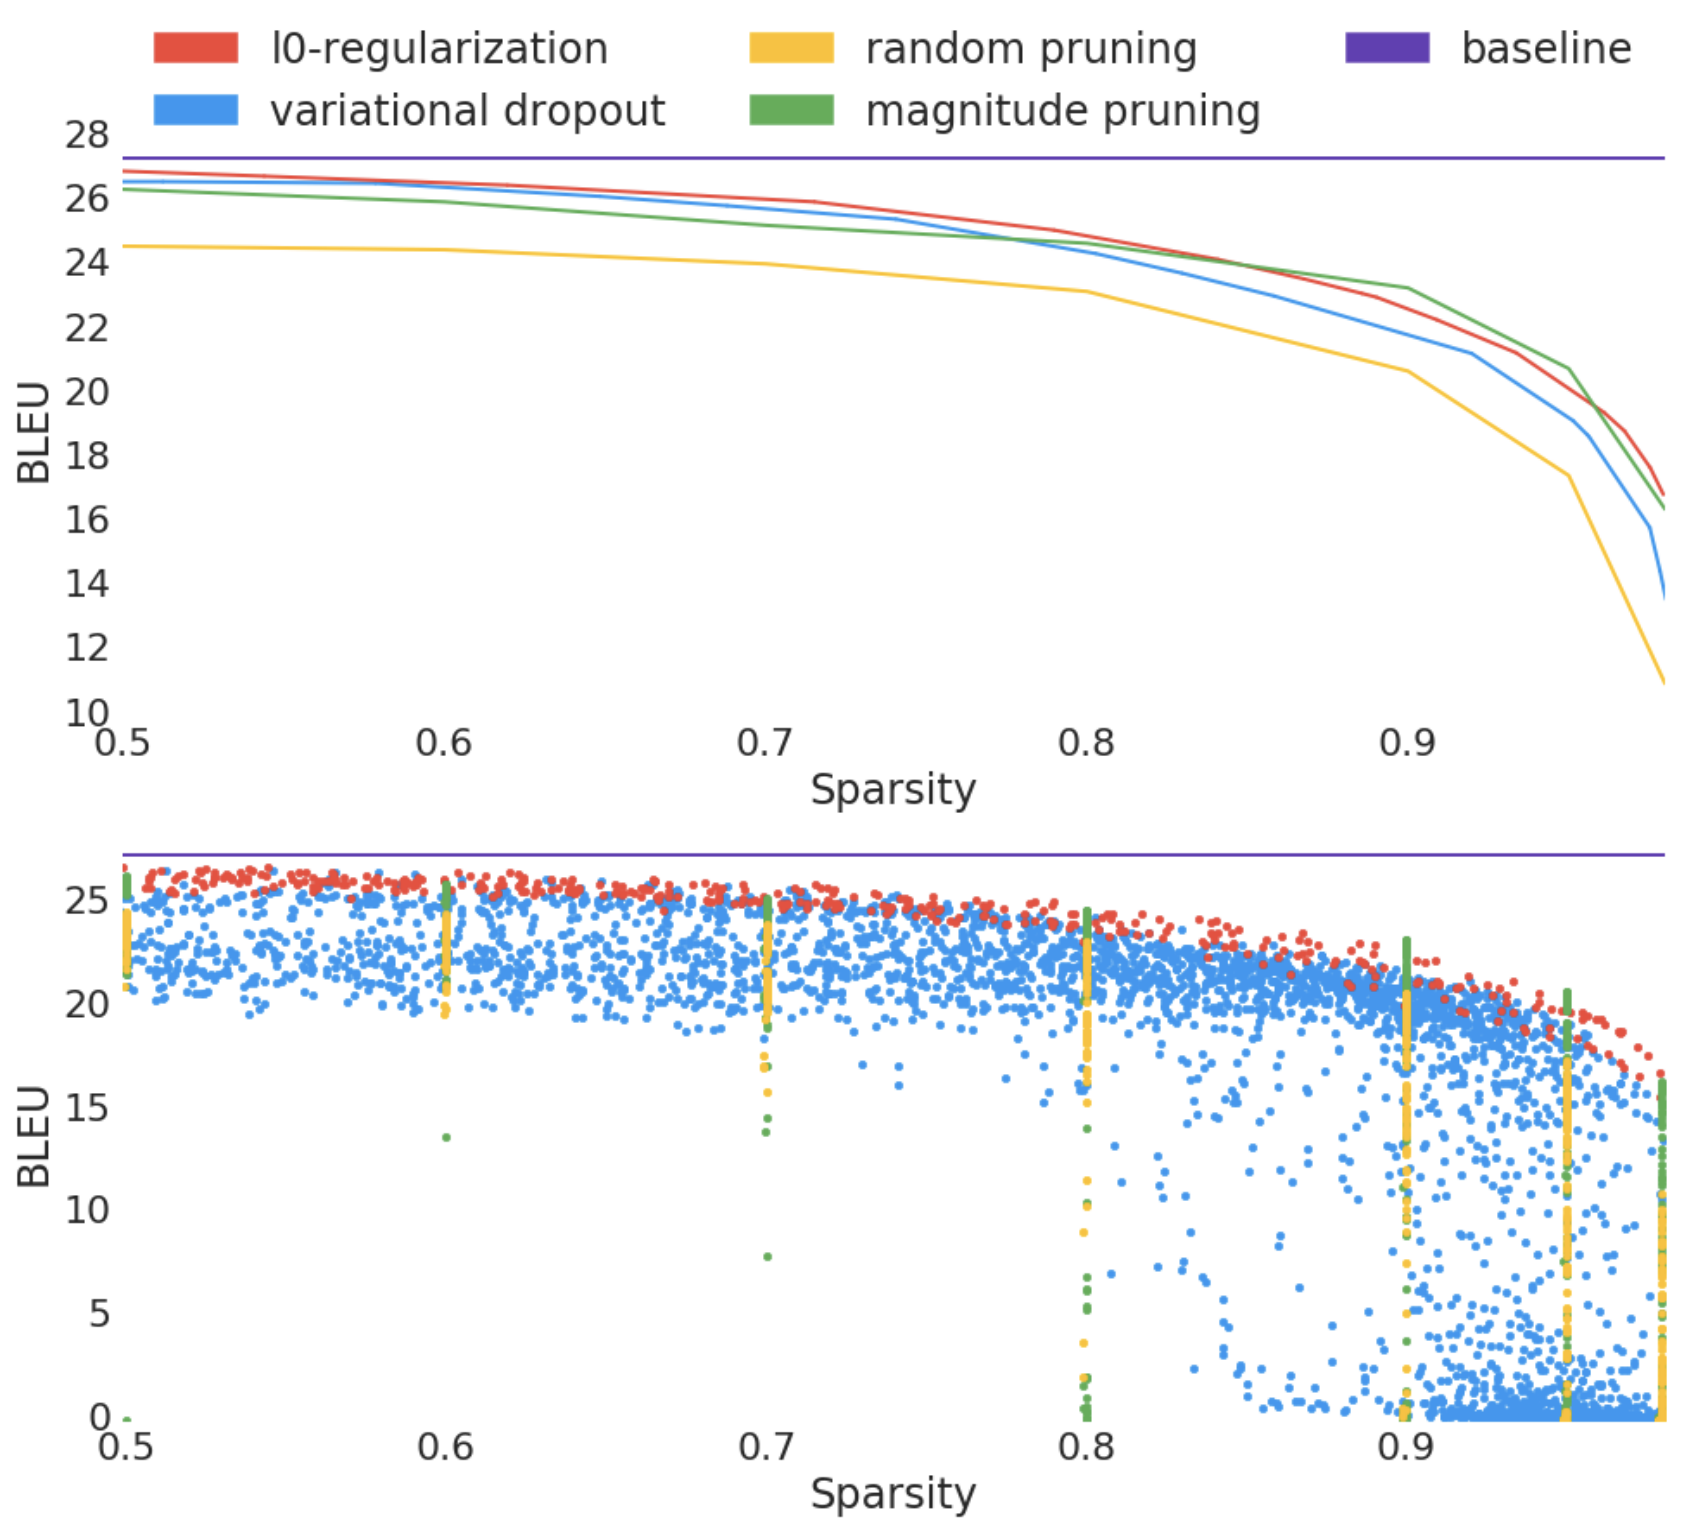
\includegraphics[width=0.6\textwidth]{images/sparsity-nmt.png}
\end{figure}

    \begin{itemize}
        \item Magnitude pruning prunes layers uniformly regardless of their type, vardrop and l0-reg prunes some layer types less aggressively
        \item Magnitude pruning outperforms vardrop and l0-reg in high-sparsity scenarios
    \end{itemize}
\end{frame}


\begin{frame}{Accuracy/sparsity tradeoff for ResNet-50 on ImageNet}
\begin{figure}
    \centering
    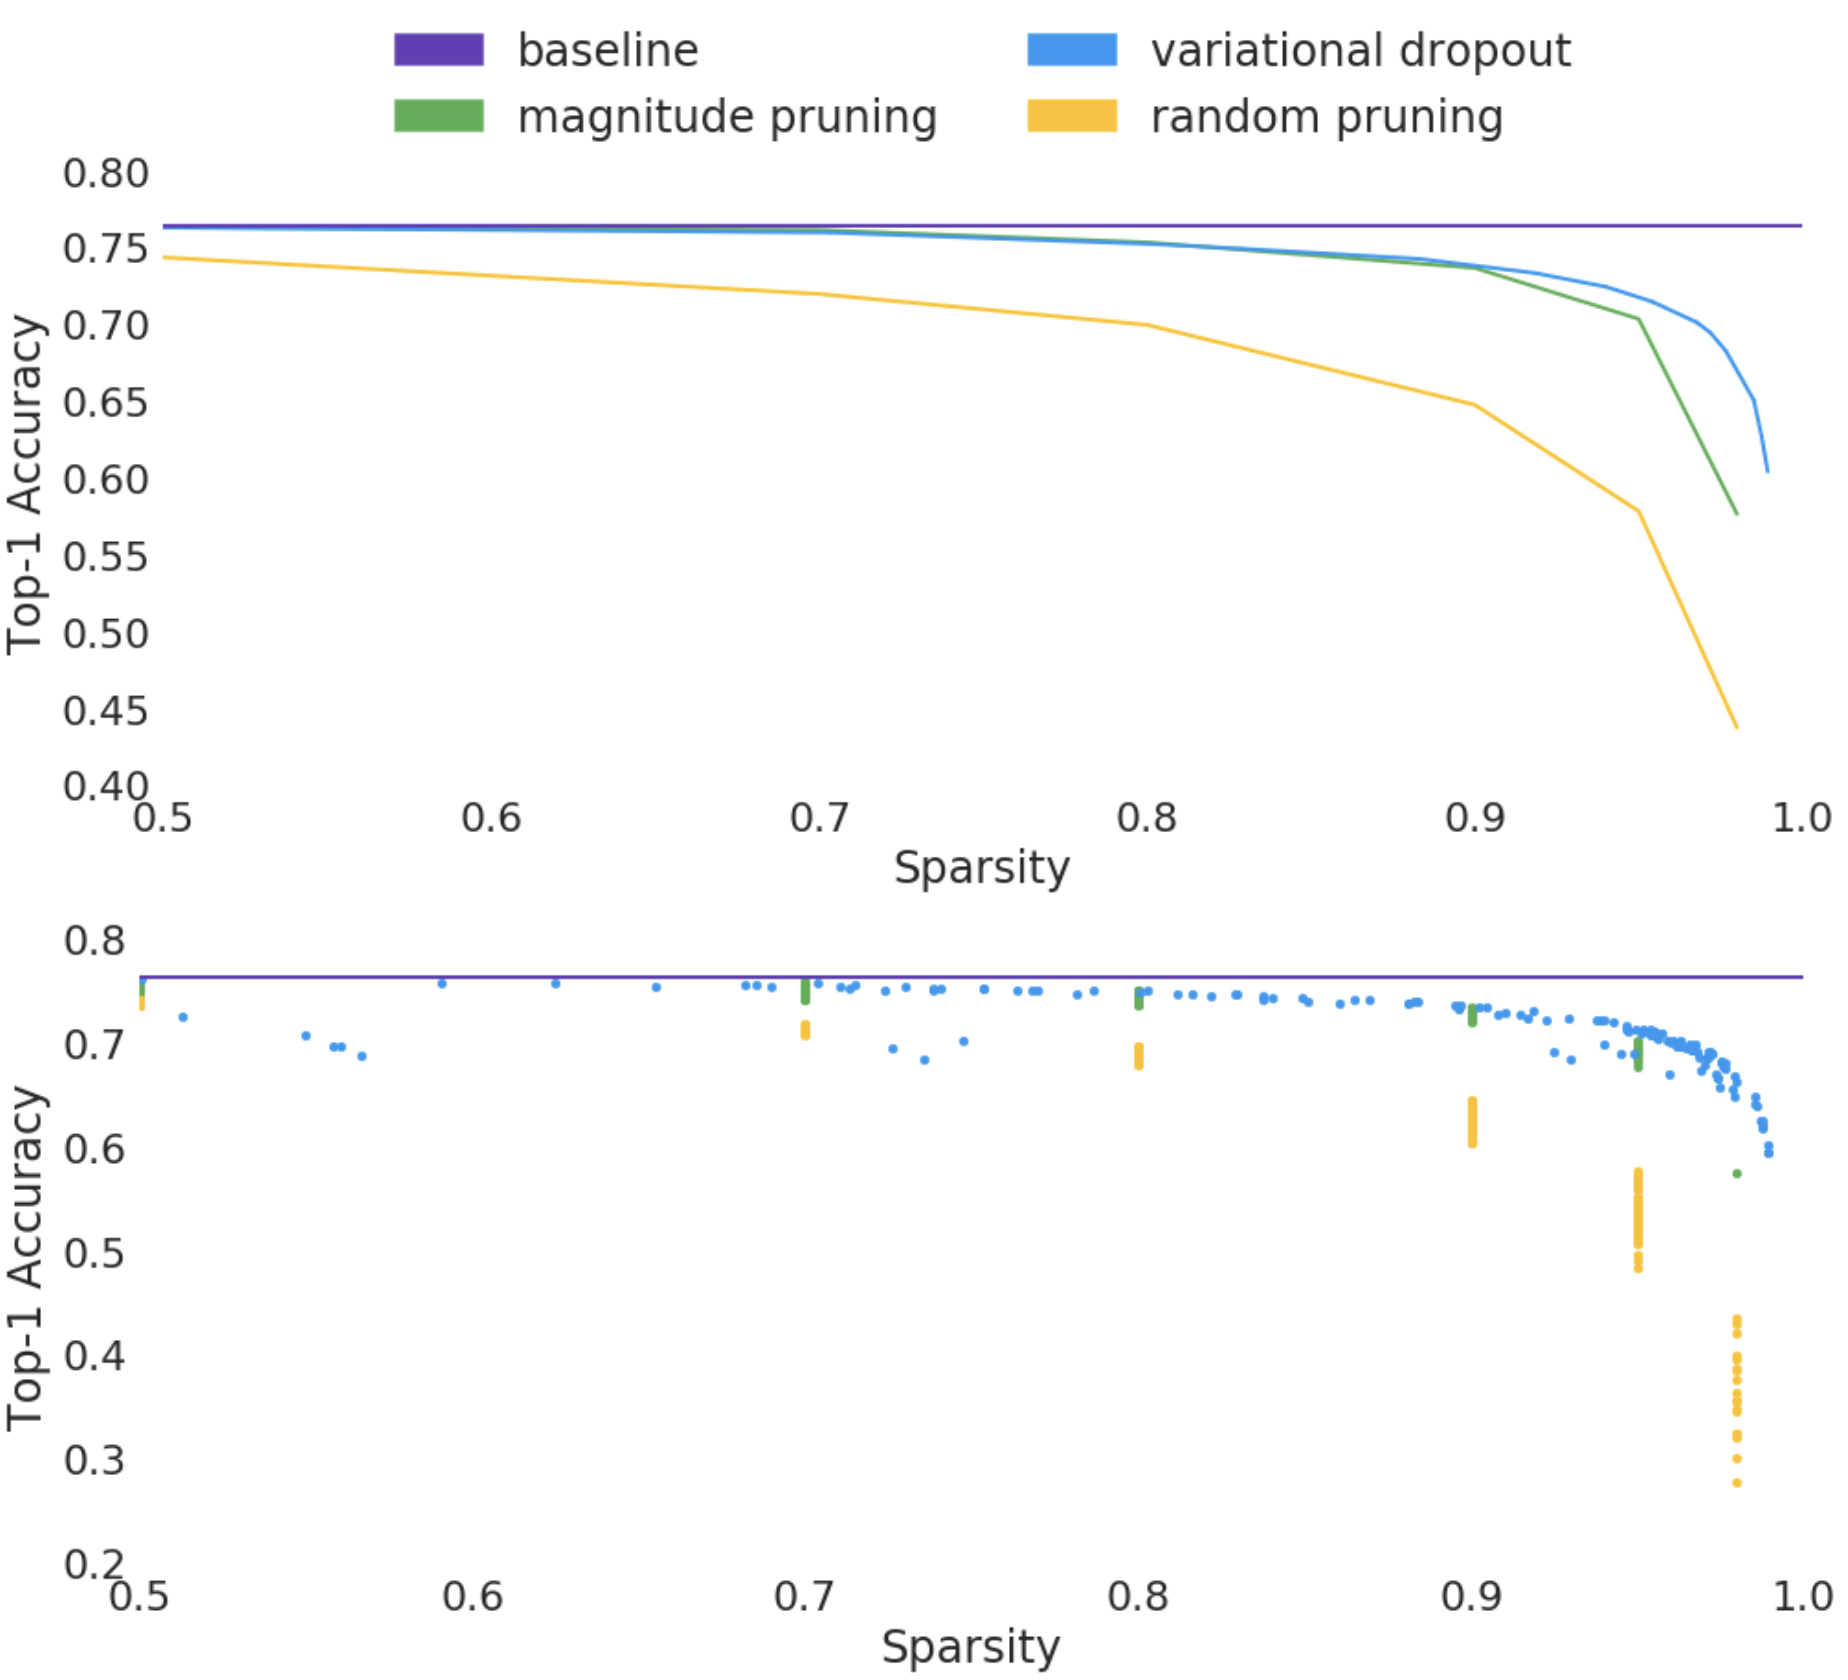
\includegraphics[width=0.6\textwidth]{images/sparsity-imagenet.png}
\end{figure}

\begin{itemize}
    \item Authors couldn't manage to make l0-reg work for this setup
    \item Vardrop worked really well (but consumes much more memory)
    \item Authors tried not to prune the first layer for magnitude pruning and it outperformed vardrop everywhere except for extreme sparsification values
\end{itemize}

\end{frame}


\begin{frame}{Testing LTH}
\begin{figure}
    \centering
    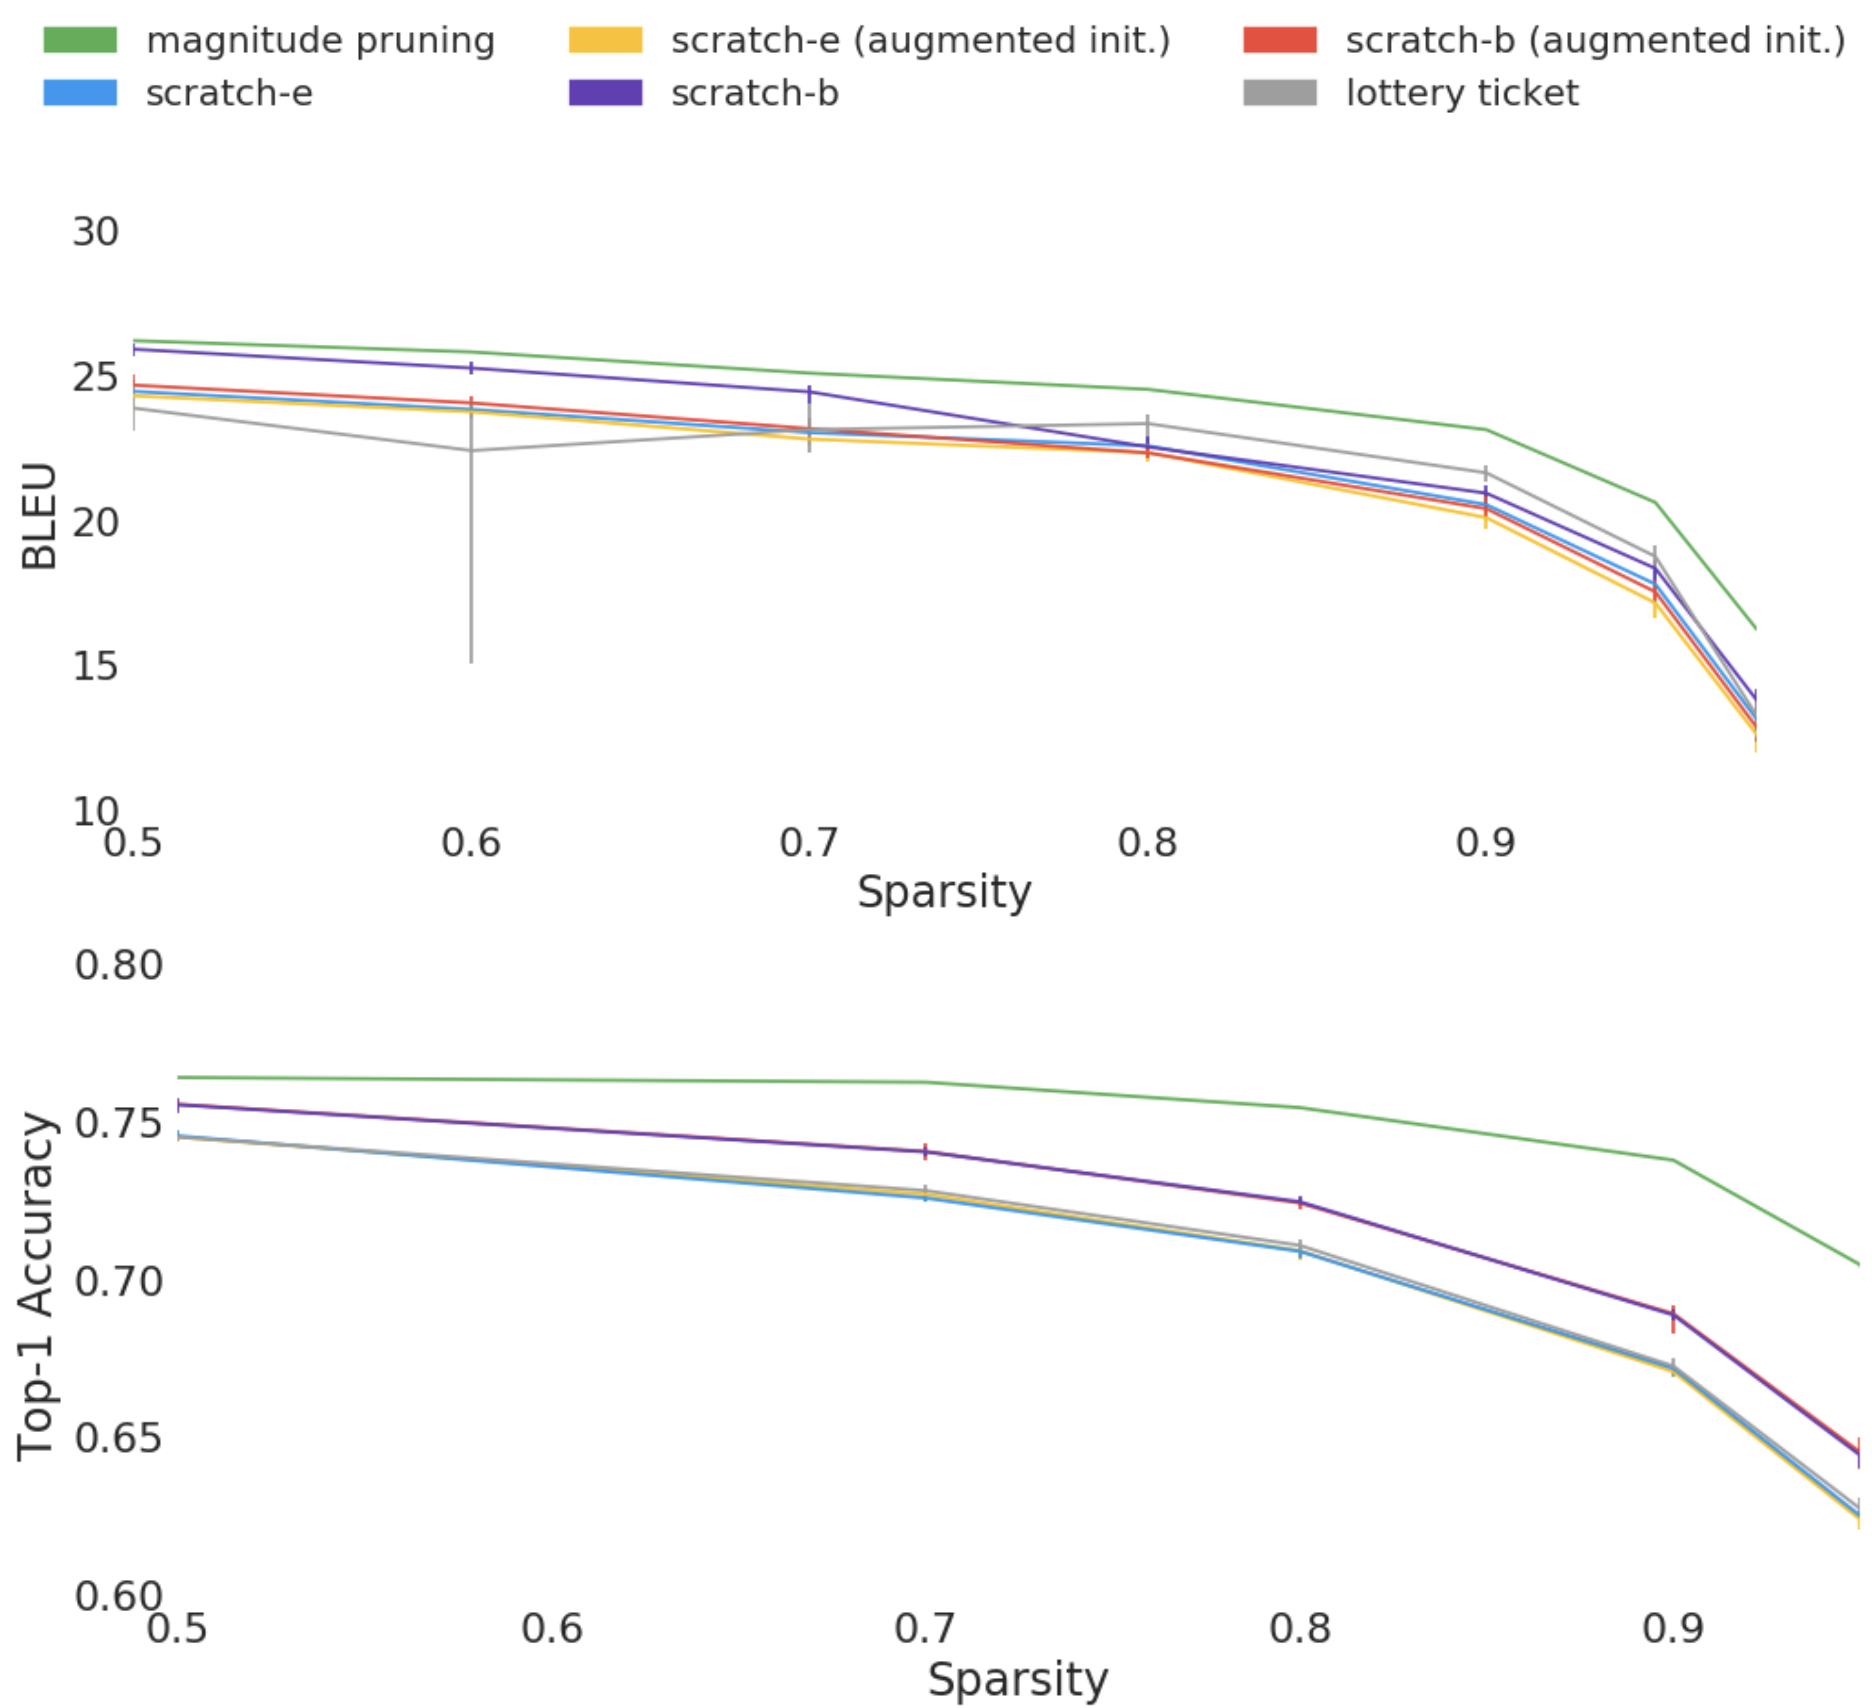
\includegraphics[width=0.6\textwidth]{images/sparsity-lth.png}
\end{figure}

\begin{itemize}
    \item scratch-e: apply the learned mask, reinit the subnetwork and retrain
    \item scratch-b: increase the number of training steps up to 2x
    \item lottery ticket: like scratch-e, but use original init
    \item augmented init: scale the variance at init by the number of non-zeros
\end{itemize}
\end{frame}


\begin{frame}{Conclusion}
    \begin{itemize}
        \item Modern SotA pruning techniques do not work that well on large-scale tasks
        \item LTH outperformed random init only for high-sparsity and only for Transformer
        \item Different pruning techniques prune layers non-uniformly, i.e. this implies and some layers are more important (for example, the initial layer and the last one)
    \end{itemize}
\end{frame}

\end{document}
